%\noindent Experiment N\textsuperscript{\underline{o}} Sxxx Safety Report\\
%TBA : EMMA PGAC detector test\\
%\\
\title{EMMA PGAC Detector Test\\ Safety Report}
\author{}
\date{}
\maketitle
\noindent Experiment Leader/Safety Coordinator:
\begin{changemargin}{\parindent}
\noindent Jon Lighthall\\
TRIUMF\\
4004 Wesbrook Mall\\
Vancouver, BC V6T\,2A3\\
Canada\\
%\href{callto:6042221047p6859}
{(604) 222-1047 x6859}\\%+44 1904 322221\\
\href{mailto:lighthall@triumf.ca}{lighthall@triumf.ca}\\
%Local Contact: -Gordon Ball\\
\end{changemargin}
\pagestyle{fancy}
\rhead{EMMA PGAC Safety Report}
\lhead{}
\renewcommand{\headrulewidth}{0pt}
%\doublespacing \linenumbers
\section{Introduction}
\subsection{Experimental aim}
%Charles Barton has extensive experience over many years with the UK PHOENIX ECRIS charge%
%breeding ions source. He was the spokesperson for the ECRIS charge breeding experiment at%
%ISOLDE where the operating parameter space and optimization of the source occurred as part of a%
%larger European research grant into charge breeding ion sources. The capabilities and limitations of%
%this versatile and powerful charge-breeding ion source are well-understood by the group at York. 
%It is understood that a facility using this source will often deliver beams of radioactive nuclei to
%experimental stations along with some level of contaminants in the beam. Users of these facilities
%should then have the capability to selectively and sensitively tag on the isotopes of interest.

The TRIUMF Detector Group has developed %a number of detectors for use at experimental facilities
the EMMA PGAC (Parallel Grid Avalanche Counter), a device that is designed to work with the radioactive beams
delivered by ISAC-II at TRIUMF.  The PGAC detector will be a key component of the detector suite at the focal plane of the EMMA spectrometer.
EMMA, currently under construction in ISAC-II,  is a recoil mass spectrometer 
which %uses electric and magnetic dipoles to
 separates recoils of nuclear reactions from the accelerated ion beam.  The reaction recoils and the unreacted beam will be dispersed  according to their mass/charge ratio.  By separating beam-like recoils from the unreacted beam, very weak reaction channels may be studied in the presence of very high-yield background channels.  In a similar manner, beam contaminants may also be separated.  
 
In order to measure the spatial distribution of particles at the focal plane, a position sensitive detector is required.  The EMMA PGAC is designed to measure the position of particles in the $x$-$y$ plane at the EMMA focal plane. %The PGAC will also provide an essential timing signal for EMMA experiments.
  The timing reference provided by the PGAC is used to measure the recoil time-of-flight, the recoil coincidence with ejectiles detected in the target chamber, and is used to generate the trigger for the data acquisition system.
%It is also designed to be able to be an ancillary detector to the TIGRESS array and should provide the capability to identify the Z of components of the accelerated beam of radioactive ions after scattering from the experimental target.
% is a position-sensitive gas avalanche counterThis position-sensitive detector 
%In addition, the PGAC can also provide limited energy loss information, which can be used for charge identification.
Ultimately the PGAC will form the entrance to the EMMA ionization chamber, a large-acceptance Bragg detector which will be used to provide $Z$-identification of the  recoils.
 
%, and provide position information to Doppler correction the $\gamma$-rays detected by the TIGRESS array.
\subsection{Beam test}
\begin{table}[b]
\begin{center}
\begin{tabulary}{0.5\textwidth}{R|L} 
Beamline&ISAC-I, HEBT  \\
Beam&$^{16}$O\\
Beam energy&16\,MeV (1.116\,MeV/$u$)\\
Beam intensity&6.2\,pnA or 3.9$\times10^{10}$\,pps\\
Targets& Au, $^{12}$C \\
\end{tabulary}
\end{center}
\caption{Parameters of the beam test. }
\label{beam_test}
\end{table}
The beam tests at ISAC-I aim to explore the %avalanche capability
peformance of the PGAC detector under realistic experimental conditions 
 %and record the signal pulse shapes
 over a range of pressure and voltage regimes. The specific beam parameters of the test are listed in Table~\ref{beam_test}. 
 The detector will be characterized with respect to its avalanche capability and 
% The performance of the detector under multiple-hit conditions will also test the 
position reconstruction capability.  These characteristics will be assessed by measuring the timing resolution and position resolution of the detector. 
%of the detector.
The experiment will be performed in the ISAC-I experimental hall and will utilize the scattering
chamber mounted at the end of the HEBT beamline. The PGAC will be mounted on an exit port of
the scattering chamber that is at an angle of 30$^\circ$ with respect to beam direction as measured
from the center of the scattering chamber.

With a beam of $^{16}$O at 1.116\,MeV/$u$, we plan to  study the elastic %Rutherford 
scattering of beam ions off a target foil into the PGAC. The scattered beam will illuminate 60\%  of the active area of the PGAC, providing test conditions which are required to fully commission the PGAC.  The beam will be tuned through an aperture %located
on a  rotating  target wheel and monitored by a Faraday cup mounted in the 0$^\circ$ exit port of the
scattering chamber.  The feedthrough for the target wheel is located off-center of the scattering chamber, however the target wheel itself will be installed on an extension arm such that the targets will be at the center of the scattering chamber. 
During the test, the beam will be focused onto one of two targets; either a 250\,$\mu$g/cm$^2$ gold target or 253.5\,$\mu$g/cm$^2$ carbon %deuterated polyethylene (C$_2$D$_4$)$_n$
 target.  Both targets will be mounted on the target wheel. The gold foil will be used initially to provide an unambiguous spectrum.  The carbon foil may be used in the latter portion of the tests to provide a more complicated spectrum, covering a wider range of energies.

Mounted on the $30^\circ$ exit port of the scattering chamber, the %active area
anode of the first PGAC will be 685\,mm from the target wheel.  With the center of the detector located at $30^\circ$ relative to the beam, the detector will cover 23.3$^\circ$--36.7$^\circ$, subtending 20.3\,msr in the laboratory.  Given an ion drift time in the PGAC of about 2\,$\mu$s, the desired maximum count rate in the detector is 250\,kHz.  Scattering from the gold foil, this count rate corresponds to a beam rate of $3.9 \times 10^{10}$\,pps or 6.2\,pnA. %   Scattering from the carbon foil, this count rate corresponds to a beam rate of 40.8\,pnA.
%Beam rates from $1\times10^5$\,pps up to $1\times10^8$\,pps will be requested to test the detector from a few 100\,counts/s up to the expected saturation rate of $1\times10^5$\,counts/s. 
With the inclusion of the 10.16\,cm diameter beam pipe, % and the proposed mask,
the detector will cover scattering angles of 25.8$^\circ$--34.2$^\circ$, subtending 12.1\,msr or 60\% of the active detector area. With the additional inclusion of the proposed mask, the exposed area is reduced by an additional 73\%.   Thus, the expected count rate is $1.0 \times 10^5$\,cps.



\section{Hardware}
\subsection{PGAC Detector}
The EMMA PGAC is a position-sensitive, multi-wire proportional counter operating in the avalanche regime. Some of the relevant specifications of the detector are listed in Table~\ref{detector}.  Two identical PGACs have been constructed and both with be tested simultaneously in the same PGAC box during these tests.  Two detectors are required for these tests in order to provide a mutual time reference.  In addition, using two detectors allows ray-tracing of the incident particles.


\begin{table}[t]
\begin{center}
\begin{tabulary}{1.0\textwidth}{R|L} 
%\begin{tabular}{p{0.45\columnwidth}|p{0.45\columnwidth}} 
\raggedleft PGAC box internal volume & 12.6\,L\\
\raggedleft $0^\circ$ scattering chamber internal volume & 50\,L\\
\raggedleft Operating pressure range&3--6\,Torr\\
\raggedleft Maximum quantity of isobutane in PGAC box (6\,Torr)&0.25\,g\\
\hline
\raggedleft Window material &Mylar\\
\raggedleft Window thickness&2\,$\mu$m\\
\raggedleft Window area& 66\,mm $\times$ 166\,mm (110\,cm$^2$)\\
\raggedleft 0.9\,$\mu$m-thick window burst pressure &24\,Torr\\
\raggedleft 2.0\,$\mu$m-thick window burst pressure &57\,Torr\\
%\raggedleft Window reverse burst pressure (SiN 30\,nm)&13<P$_\textrm{rb}$<27\,mbar\\
\hline
\raggedleft Cathode wire pitch&1.0\,mm\\
\raggedleft Anode-cathode gap&3.18\,mm\\
\raggedleft Active area&60\,mm $\times$ 160\,mm (96\,cm$^2$)\\
\hline
\raggedleft Typical anode-cathode voltage &550\,V\\
\raggedleft Typical anode voltage &+470\,V\\
\raggedleft Typical cathode voltage &-80\,V\\
\end{tabulary}
\end{center}
\caption{Characteristics of the PGAC detectors and the experimental setup.}
\label{detector}
\end{table}

\subsubsection{Mechanical}
Each PGAC detector is rectangular in cross section with an active area 160\,mm in the $x$-direction and 60\,mm in the $y$-direction. The anodes of the two PGACs are separated by 30\,mm in the $z$-direction. The box containing the PGACs is 41\,cm wide, square in cross section, and 10\,cm deep.
%depth and weight bout 6\,kg.
The PGAC will be filled with isobutane at a pressure of 3--6\,Torr. The 12.6\,L internal gas volume of the PGAC box will be separated from the vacuum of the 50\,L scattering chamber by a 2\,$\mu$m thick Mylar window. 

The PGAC box will be mounted to the scattering chamber at the end of the HEBT beam line at an angle of 30$^\circ$ relative to the beam line.  Fig.~\ref{schematic} includes a diagram of the experimental setup and a photograph of the scattering chamber.  The PGAC will be connected to the scattering chamber by a short beam pipe.  The length of the pipe is such that the 
entire active area of the PGAC detector will be visible to beam scattered from the target
 at the center of the scattering chamber. The beam pipe will connect directly to the front of the PGAC box via an adapter plate which houses the Mylar foil. The adapter plate is shown in Fig.~\ref{photos}.

% This short beam pipe will have a flange on one end to couple it directly to the exit port of the chamber; on the other end, a flange will couple it directly to a plate on the front of the PGAC.  %Approximately 23\% of the total PGAC detector area will be exposed to scattered beam as ray-traced from the target, through the scattering chamber and coupling pipe onto the PGAC.
%\marnote{This figure should be updated!}
\begin{figure}[ht]
\centering
%\includegraphics[width=\textwidth,height=0.4\textheight,keepaspectratio]{York_PGAC_safety_rev_11c.jpg}
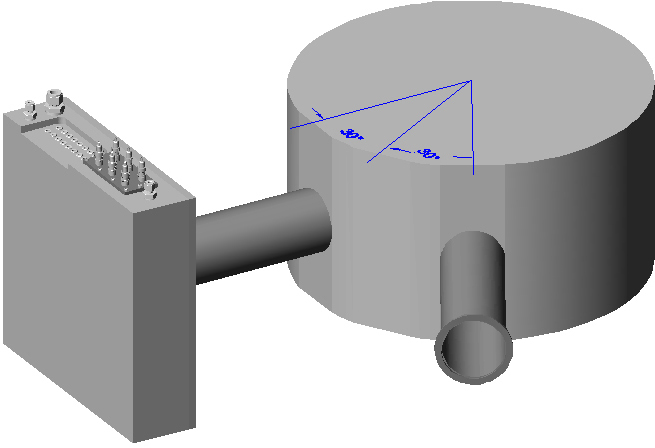
\includegraphics[width=0.48\textwidth,keepaspectratio]{HEBT_Scat_Chamber_3D_trim}\hspace{\fill}
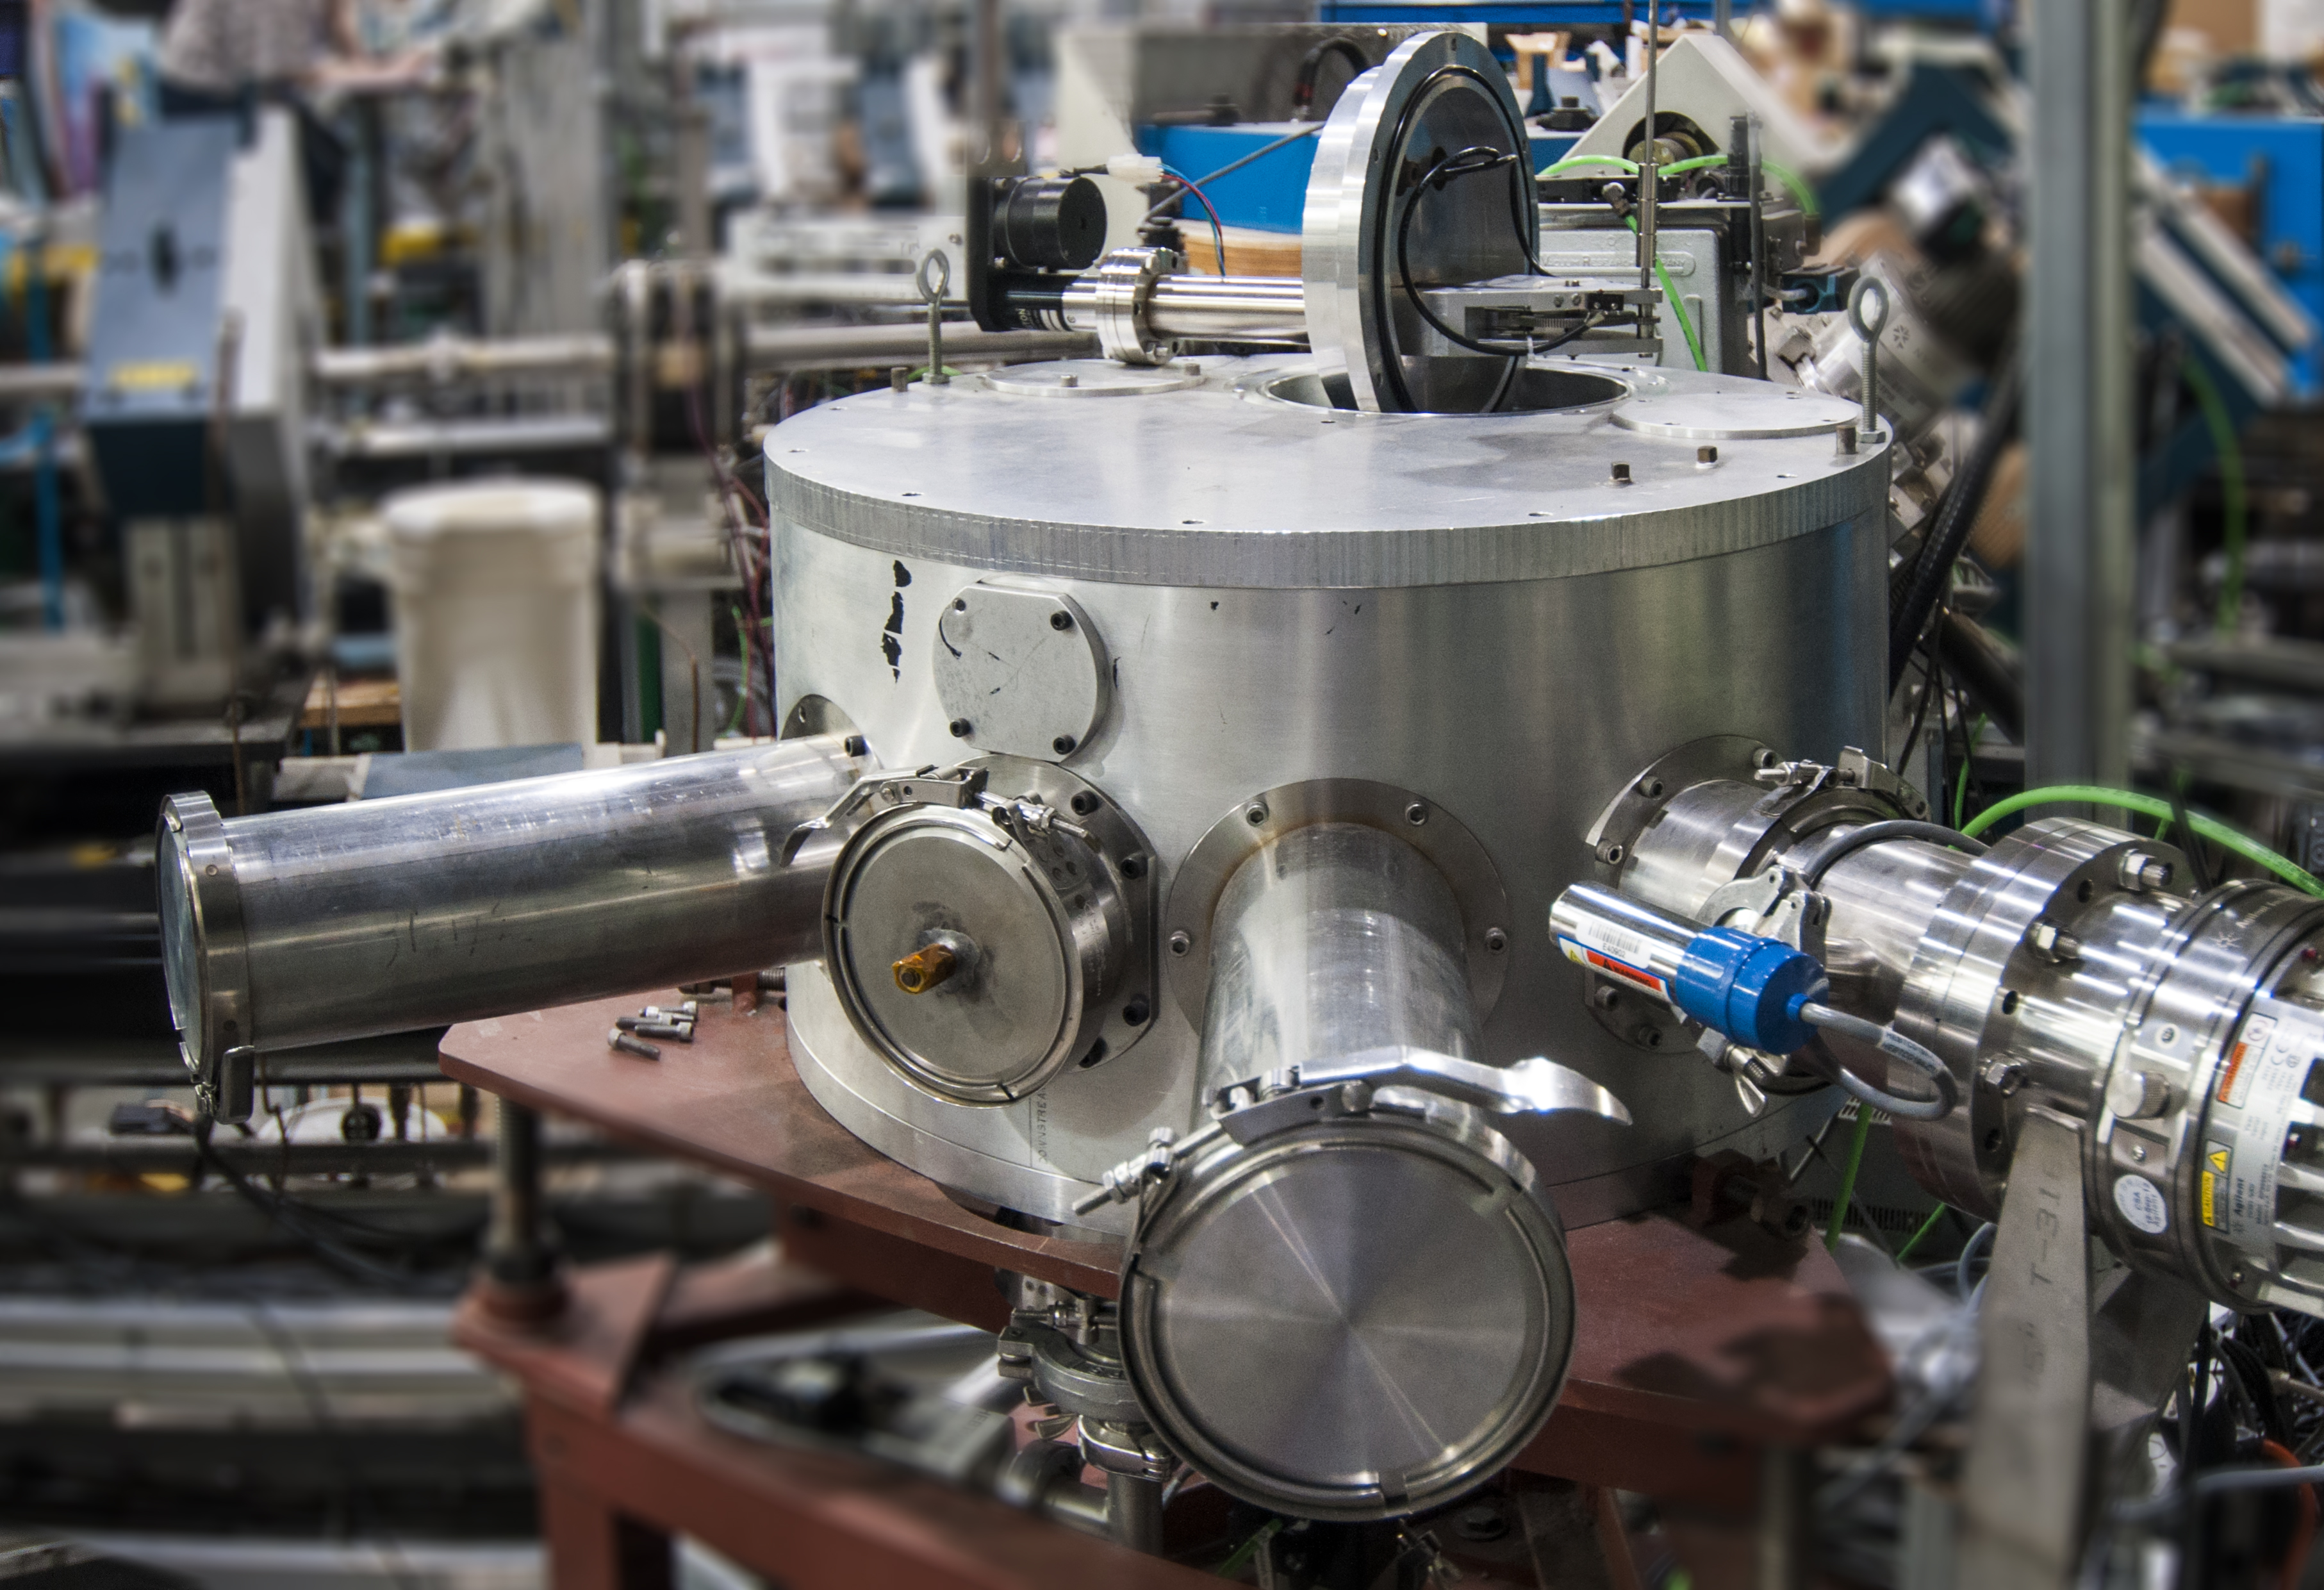
\includegraphics[width=0.48\textwidth, keepaspectratio]{DSC_0004} \hspace{\fill}
\caption{(Left) Schematic diagram of the proposed experimental setup of the 
showing a view from downstream of the HEBT beam line.  The beam enters the 0$^\circ$ scattering chamber from the top of the figure.  The beam will bombard a target foil at the center of the chamber and scattering into the PGAC box, mounted at 30$^\circ$ relative to the beam line.  The length of the beam pipe connecting the PGAC box to the scattering chamber is such that 60\% of the active area of the PGAC will be illuminated.  (Right) A photograph of the 0$^\circ$ scattering chamber before PGAC box installation.
%above %(left) and outside (right) of
%the scattering chamber. The York PGAC is shown, but the configuration of the EMMA PGAC will be similar.  The coupling flange to the PGAC, including a xx\,cm connecting pipe are shown, demonstrating the clearance of the 0$^\circ$ Faraday cup.
}
\label{schematic}
\end{figure}
\begin{figure}[ht]%
\centering
\hspace{\fill}
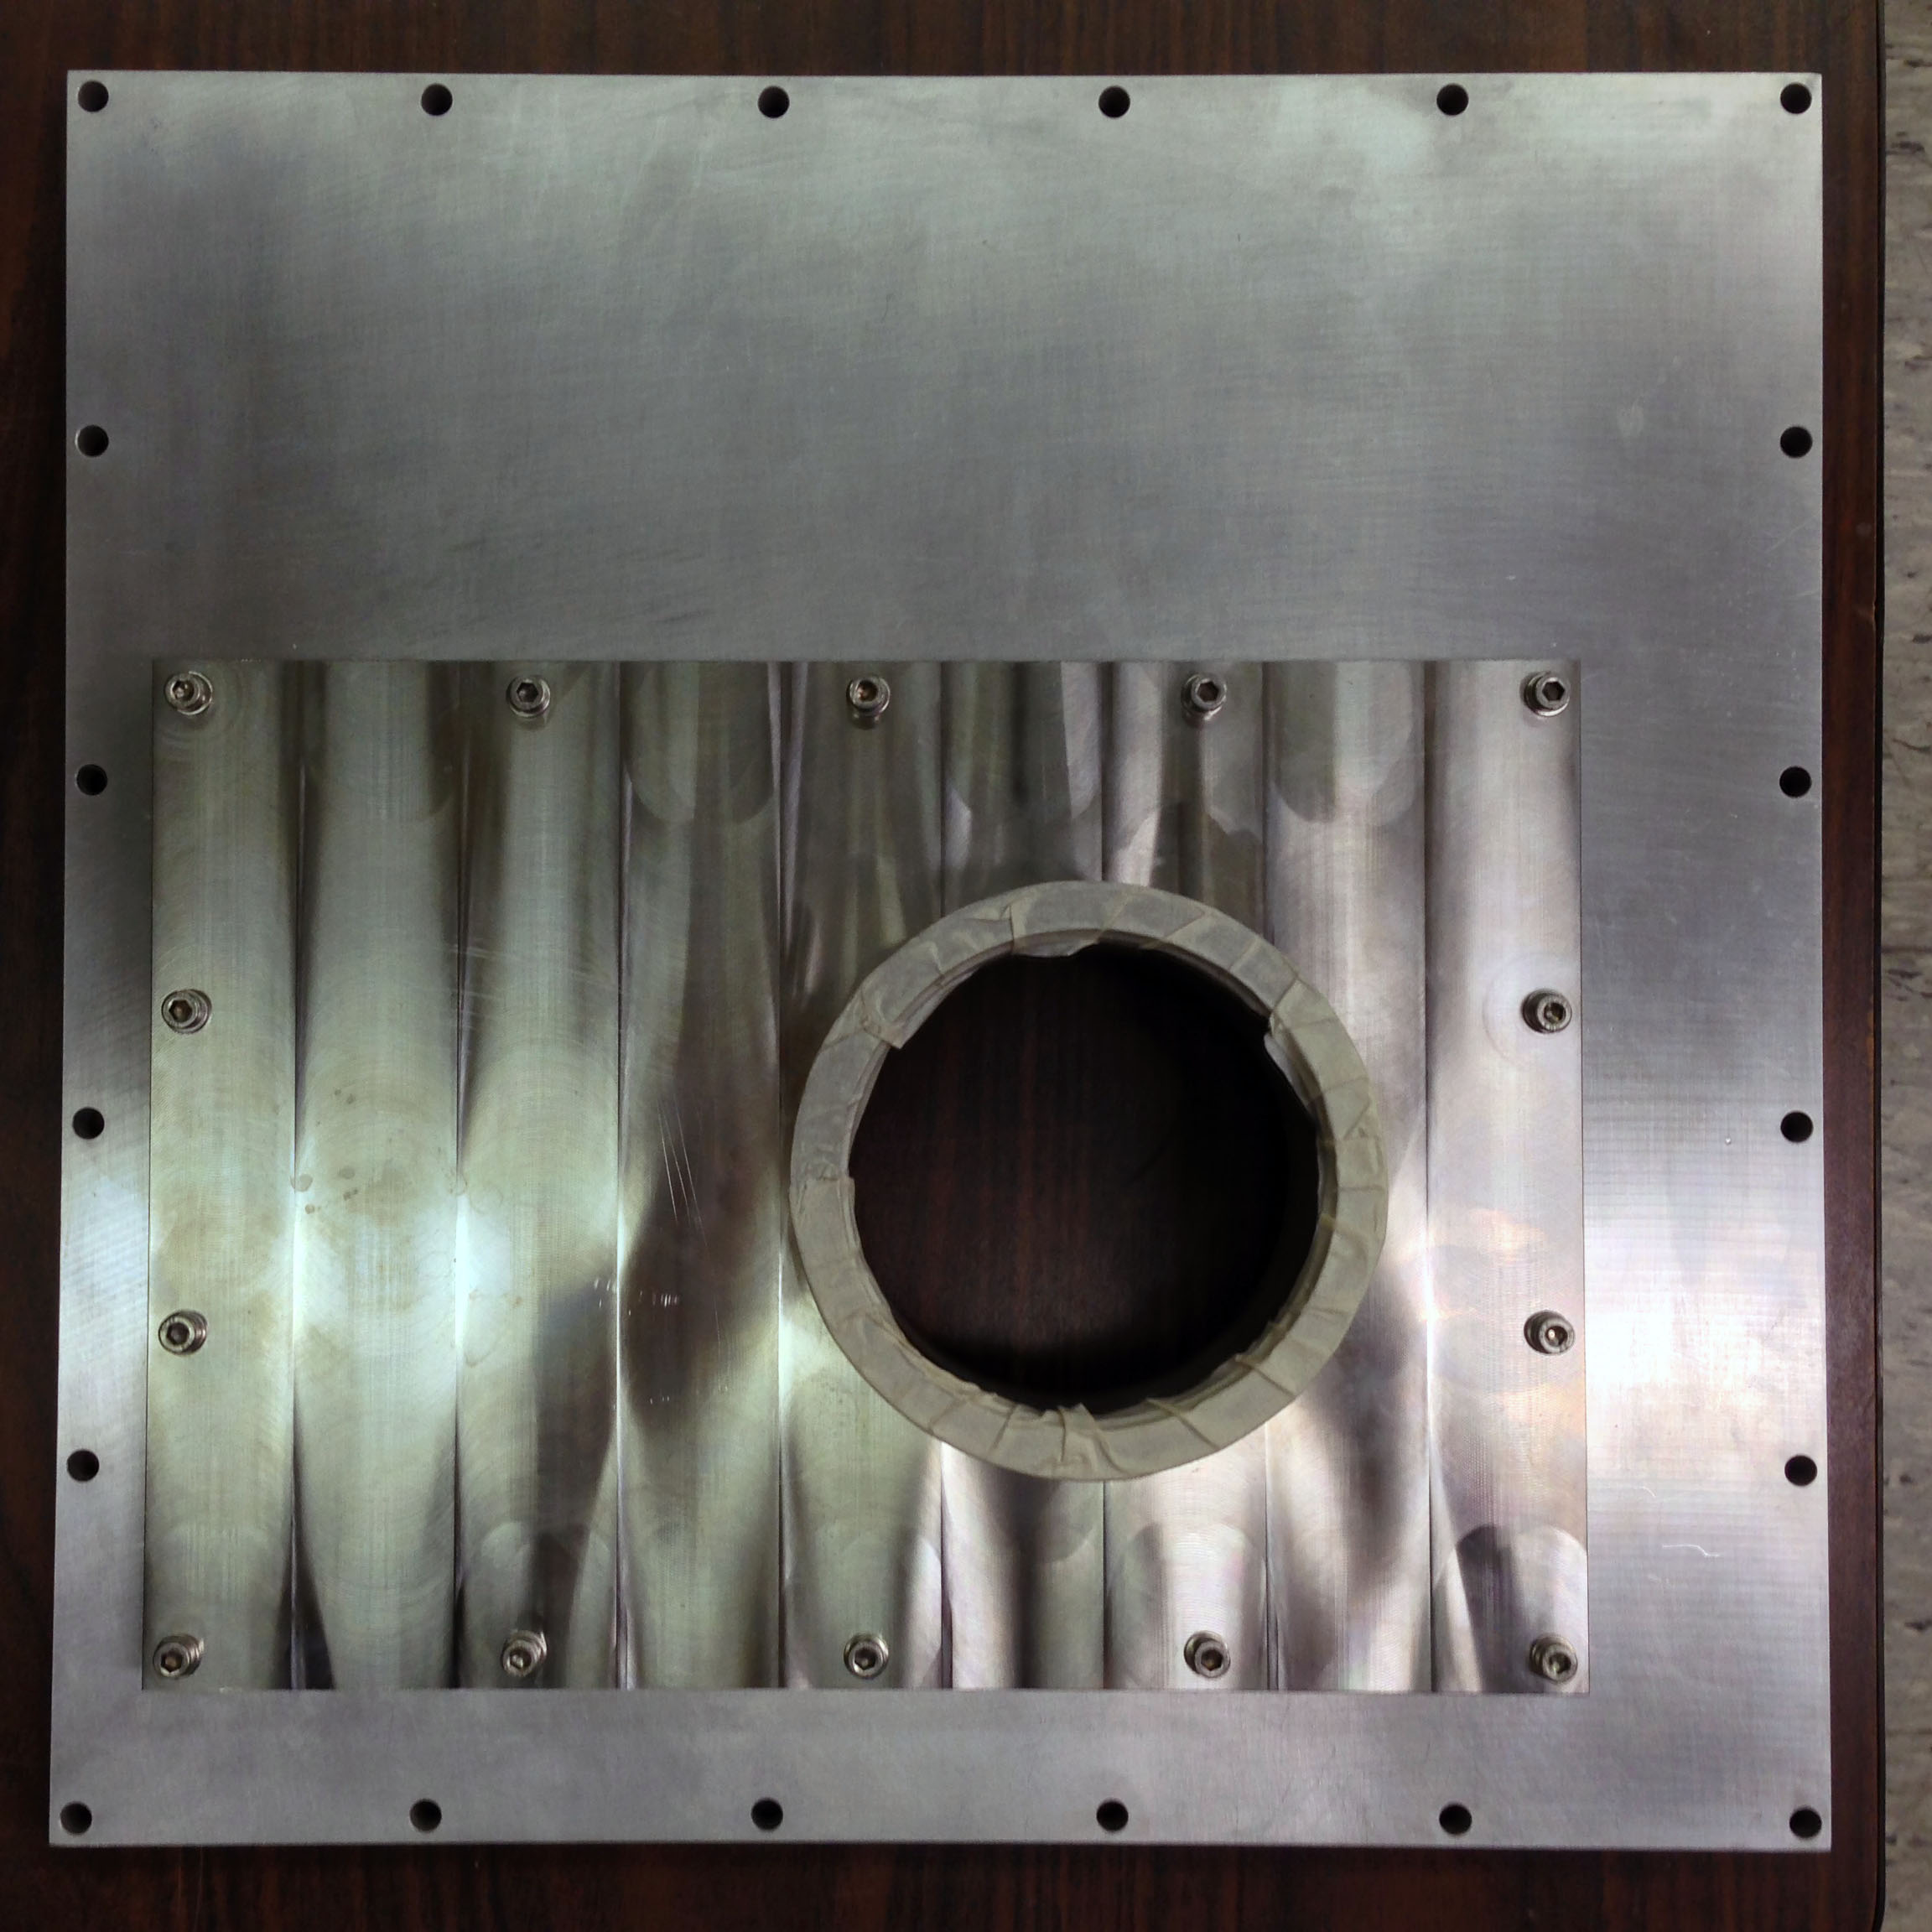
\includegraphics[width=0.48\textwidth, keepaspectratio]{IMG_0037c} \hspace{\fill}
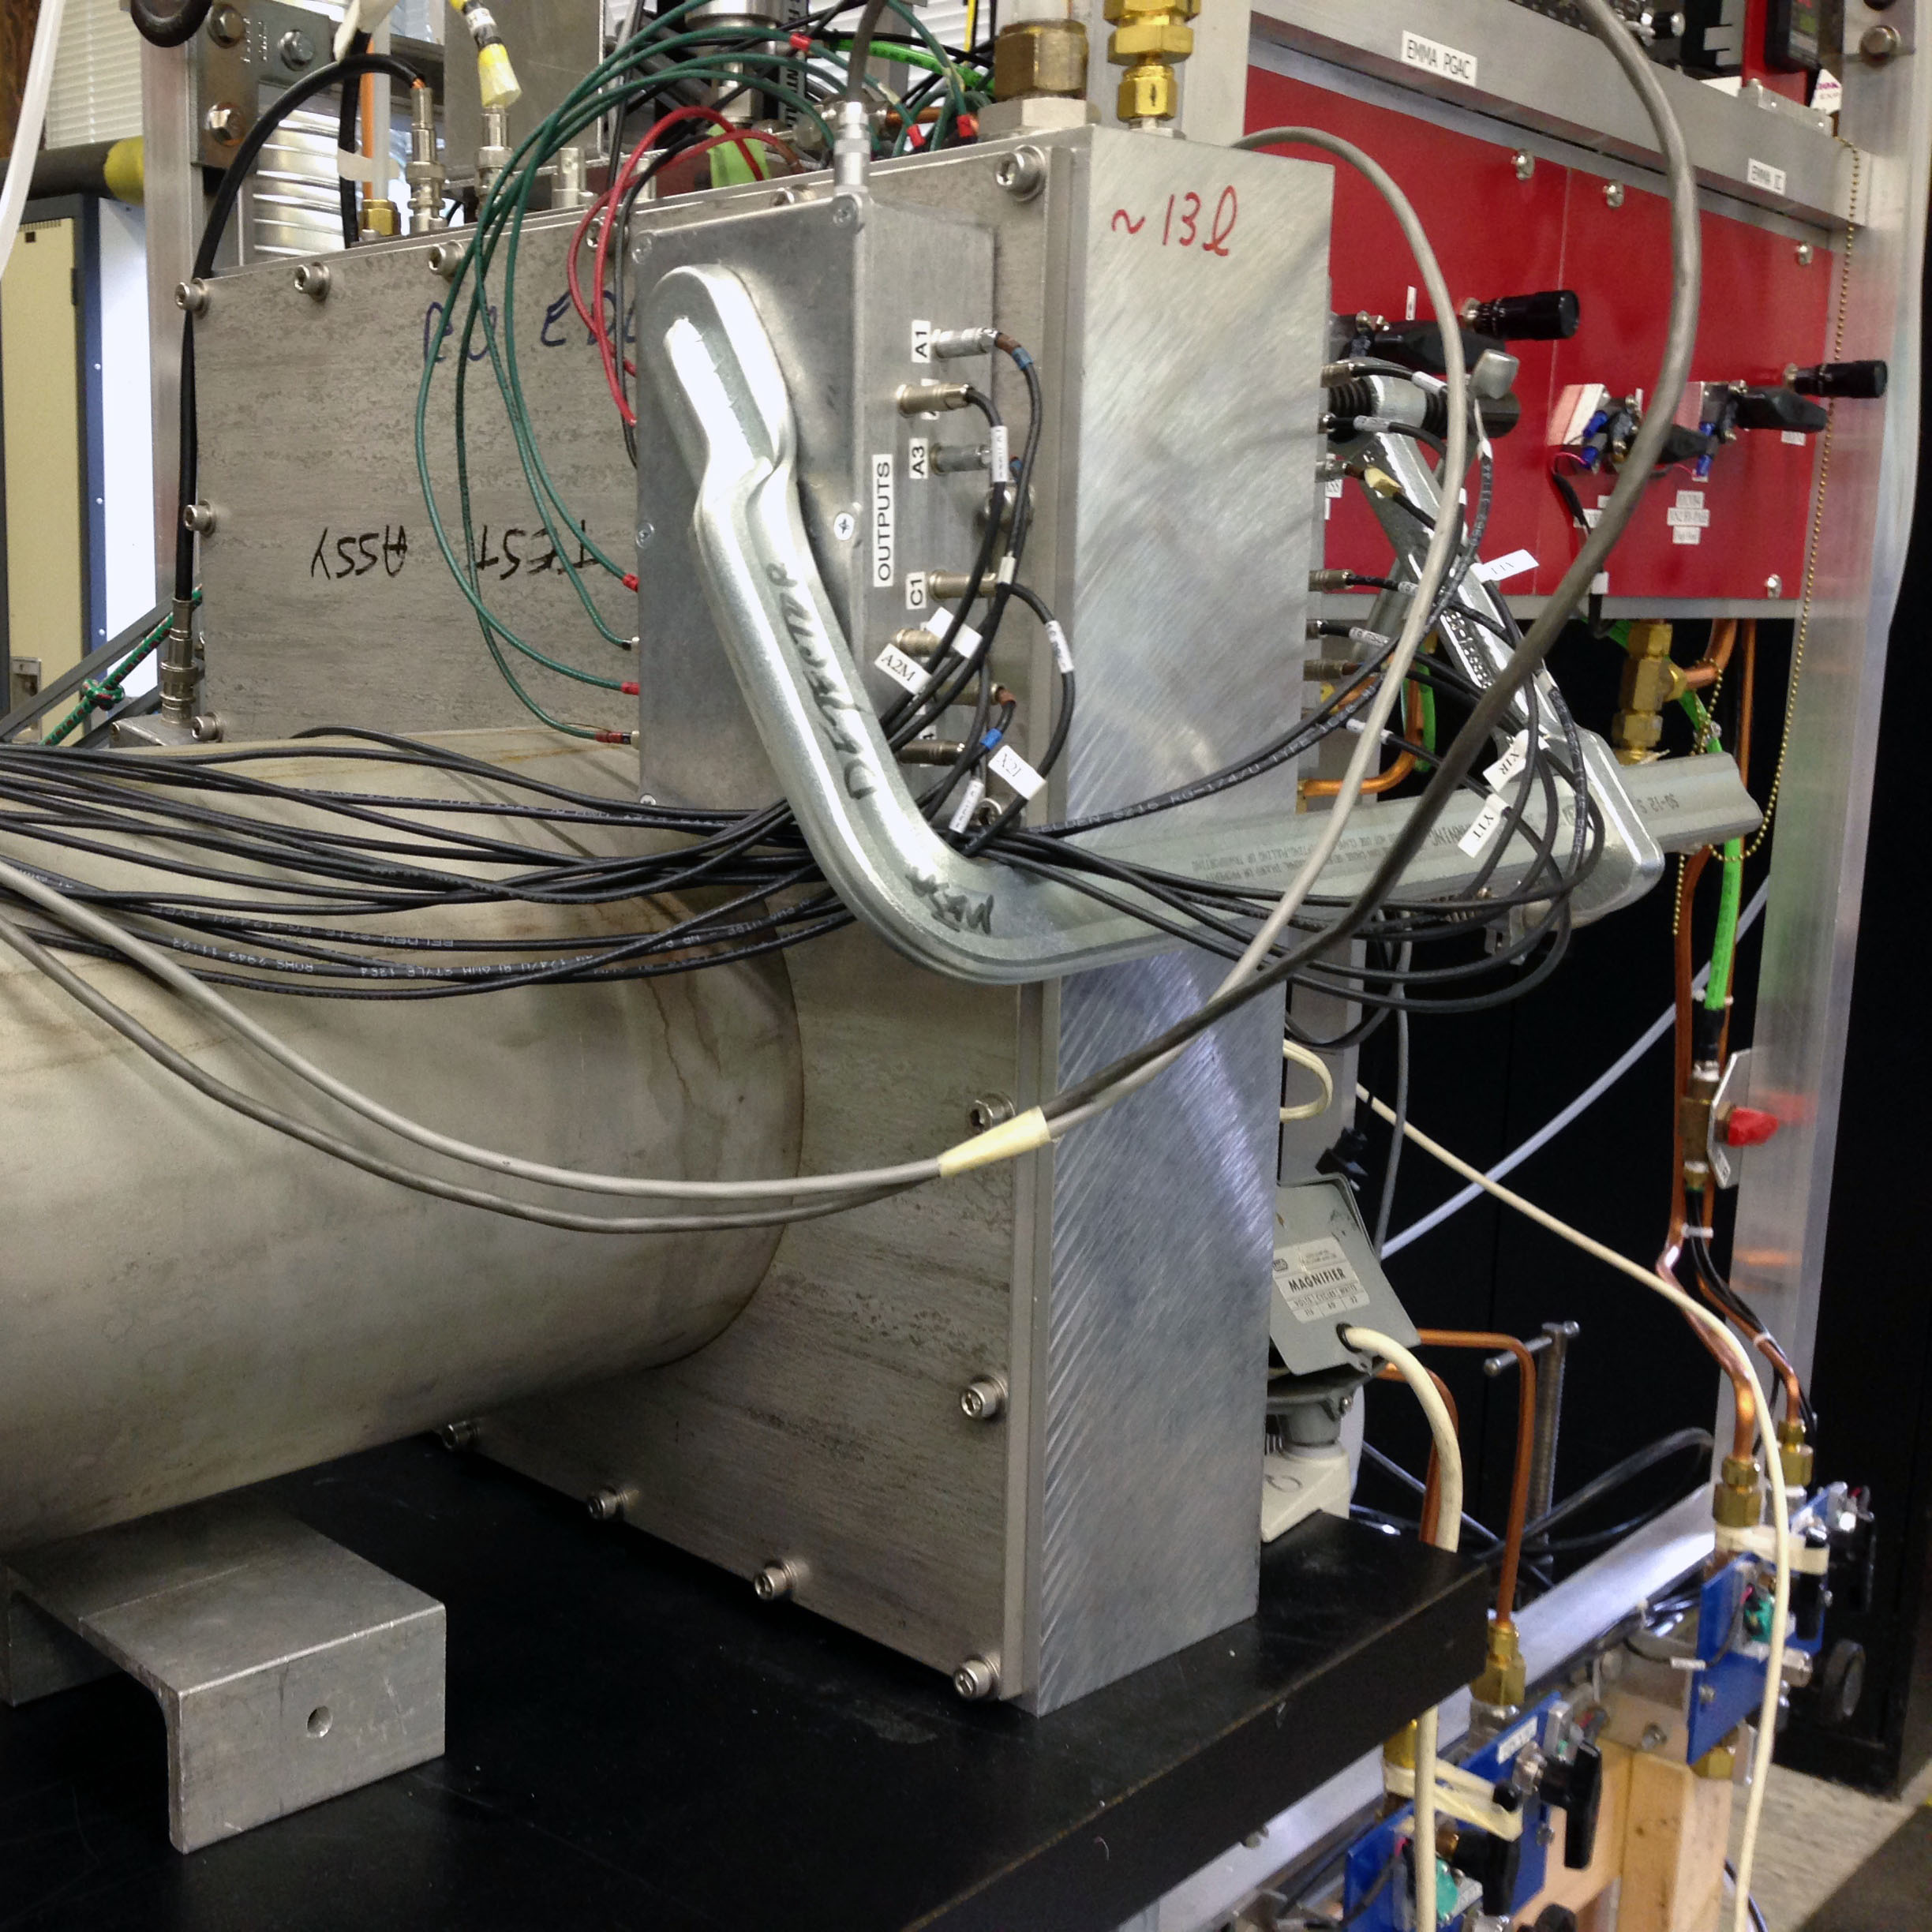
\includegraphics[width=0.48\textwidth, keepaspectratio]{IMG_0022c} \hspace{\fill}
\caption{(Left) The ``snout'' cover that will be used during the in-beam test to attach the PGAC box to the $0^\circ$ scattering chamber. (Right) The PGAC box and the gas-handing system during bench tests in the Detector Development Lab.}%
\label{photos}%
\end{figure}

\subsubsection{Electrical}
Beam scattered into the gas volume of the detector will cause ionization that will be accelerated by the %high
 voltages applied to the electrodes and multiplied by the gas into an ion avalanche.
The  voltage applied to the anode and cathode depend on the operating pressure of the detector.  At 4\,Torr, the voltage difference between the anode and cathode is typically 550\,V.  The anode is held at a positive voltage, 470\,V at 4\,Torr.  The two cathodes are held at a relatively small negative voltage, -80\,V at 4\,Torr.  The negative voltage on the cathodes is used to produce a potential difference between the cathodes and the walls of the chamber, which are at ground potential, in order to prevent the detection of ionization from outside of the active region.  

For each event, seven signals are output by each PGAC. Each cathode forms a delay line with 2.5\,ns added between adjacent cathode wires.  Signals are read from each end of the cathode with the position derived from the difference in time between the signals.  One cathode measures positions in the $x$-direction, the other measures positions in the $y$-direction, for a total of four cathode signals.
The anode is divided into three sections to reduce the capacitance of the detector and improve timing performance.  The anode signal is the characteristic timing signal of the PGAC.% and it 

All seven signals from the PGAC pass through a  %NIM mounted
pre-amplifier mounted to the chamber.  The pre-amp signals are further amplified using linear fast timing amplifiers.  The amplified signals are entered into a leading-edge discriminator to produce logic signals.  All seven logic signals are read into the acquisition system using a time-to-digital converter (TDC).  %boosts these signals
 %and the rise of the signals will be recorded with high time precision on a CAEN desktop digitizer. The digitizer must be triggered.
The logical OR of the anode signals is used to generate the trigger for the data acquisition system.%  This signal is fed into a fast leading-edge discriminator NIM module which provides the fast trigger to acquisition system.  


\subsection{Gas Handing System}
The newly-built EMMA gas handling system (GHS) will be used for the PGAC detector tests.
The gas handling system is designed to provide a stable flow of isobutane gas to the EMMA PGAC.  The hazards related to isobutane are discussed in \S\,\ref{flame}. The nominal volumetric flow rate is Q=60\,cc/min with Q$_\textrm{min}=20$ and Q$_\textrm{max}=100$.
The gas handling system must also maintain a constant set pressure  in the PGAC volume. The nominal operating pressure of the PGAC is 4--6\,Torr.
A schematic diagram of the vacuum and gas handling system  is shown in Fig.~\ref{diagram}. 
The primary design considerations for the EMMA PGAC GHS are to:

\begin{itemize}
\setlength{\itemsep}{0pt}
\setlength{\parskip}{0pt}
\setlength{\parsep}{0pt}
	\item Provide a stable operating pressure in the PGAC box
	\item Prevent a rupture of the thin PGAC window due to differential pressure during normal operations and during pumping and venting procedures
	\item Avoid flammable mixtures of air and isobutane
	\item Avoid the ignition of any flammable mixtures formed
	\item Protect the beam line vacuum from any rupture of the PGAC window
\end{itemize}

Isobutane is supplied from cylinders in the ISAC Gas Handling Building. The maximum flow into atmospheric pressure in the ISAC-II area is limited to 250\,cc/min by a low-pressure regulator feeding gas through a pre-set needle valve. The air-actuated valve \texttt{VA1} on the supply line 
is used to isolate the PGAC from the gas system when certain pressure interlocks are tripped and during pump-out and venting procedures.  On the  exhaust line, the PGAC is isolated by turning off pump \texttt{PU1} which automatically closes the pump valve.
\hyphenation{pro-por-tion-al}
Pressure control is provided by absolute pressure transducer \texttt{PA1}, flow controller \texttt{FC1} and the PID (proportional-integral-differential) controller. The PGAC pressure measured by \texttt{PA1} is input to the PID, which then outputs a signal to adjust flow through \texttt{FC1} such that the PID set-point pressure is maintained. %The flow out of the chamber is set by adjusting needle valve \texttt{VN1}.
 Differential pressure transducer \texttt{PD1} measures the pressure between the PGAC and the scattering chamber, e.g., the pressure across the PGAC window.% and is used to trigger interlocks if the differential pressure (in either direction) across the window exceeds threshold levels either during normal operation, or during filling and venting procedures.

Control of the flow of isobutane out of the PGAC chamber is  provided by precision needle valve \texttt{VN2} on the exhaust line upstream of scroll pump \texttt{PU1}. Ball valve \texttt{VB2} provides a large orifice bypass around \texttt{VN1} to allow efficient pumping to \texttt{VB6} for leak tests, and to allow efficient evacuation of isobutane from the PGAC prior to venting the system with air.

%Air-actuated valve \texttt{VA2} connects the PGAC volume to the diagnostic box during pump-out and venting procedures. \texttt{VA2} can also be forced open by a differential-pressure interlock to prevent destruction of the PGAC window from large differential pressure. This interlock only occurs, if other interlocks which are triggered at lower differential pressure have failed to remedy the situation. An interlock prevents \texttt{VA2} from being open if either or both of the gate valves \texttt{SEBT2IV2} and \texttt{SEBT2IV3} are open.

%\begin{landscape}
%\centering
%\vspace*{\fill}
\begin{figure}[t]
%\vspace*{-1in}
%\centering
\centerline{
\includegraphics[width=\columnwidth]{EMMA_ISAC1_GHS_1%
%logic_v6
}
}
\caption{Schematic diagram of the gas/vacuum handling system for the EMMA PGACs.
%Devices shown above the diagnostic box are all gas system devices. Devices shown below the diagnostic box are all normal vacuum system devices in the HEBT beam line.
%Modifications to the existing gas system will be required and are indicated in blue.
}
\label{diagram}
\end{figure}
%\vspace*{\stretch{1}}
%\vfill
%\end{landscape}

Gas will be supplied from the ISAC gas shack through stainless steel flammable-gas lines where the
flow rate of the line is limited to 250\,cc/min into atmosphere. The gas exhaust from the
PGAC box will be pumped through roughing pump \texttt{PU1}, separate from the HEBT vacuum system, that will evacuate the detector gas through a gas exhaust line back to the gas shack.
The presence of the 2\,$\mu$m-thick Mylar window at the entrance of the PGAC box requires bypass valve \texttt{VB4}
to maintain a differential pressure within $\pm 4$\,Torr between the volume of the PGAC box and the volume of  the 0$^\circ$ scattering chamber
during pumping and venting procedures.

\subsection{Status}
The PGAC detector has been designed, built and tested by the TRIUMF Detector Development group.  The next phase of commissioning requires in-beam testing to commission the detector for in-beam use. % and is ready for beam tests for the next part of the commissioning procedure.
The PGAC is designed to be operated with heavy ion beams.  The ionization potential of $\alpha$-decay sources, such as the $^{241}$Am source used in the bench tests,  is insufficient to adequately test the performance of the detector.  For example, with the detector optimized for $\alpha$ particles at 5\,Torr, the signal-to-ratio is %3--4:1
2.7:1  for the cathode, 10.9:1 for the andode,
 and the timing resolution is 1.8\,ns~FWHM.  %The jitter induced by the slow rise times of the weak signals
The ionization from the scattered $^{16}$O beam will be a factor of 12.1 greater than the ionization from the $\alpha$ particles from $^{241}$Am. The robust signals produced by the $^{16}$O will improve the timing resolution by about a factor of 3 and provide a more accurate characterization of the detector.  In-beam testing will also allow a more thorough examination of the position reconstruction and 
maximum incident particle rate.

The EMMA PGAC test will utilize the same interlocks and safety systems implemented on the HEBT beam line that were developed for the test of the York PGAC.  In addition, 
%\begin{enumerate}
%\setlength{\itemsep}{0pt}
%\setlength{\parskip}{0pt}
%\setlength{\parsep}{0pt}
%\item Convectron gauge \texttt{HEBT:CG19} has been connected to EPICS.
%\item Needle valve \texttt{MVV19} has been installed downstream of valve \texttt{HEBT:VV19} to control the vent rate and protect the
%PGAC window.
%\item Interlock valve \texttt{VA1} has been installed.
%\item A flammable gas sensor has been installed, commissioned, and calibrated in the experimental area.
%\item The Controls group has provided a ``digital out'' port for valve \texttt{VA1},
%a ``digital out'' port for the HV interlock, and an ``analogue in'' port for \texttt{FC1} flow signal.
%\end{enumerate}
the following hardware changes must be made:
\begin{enumerate}
\setlength{\itemsep}{0pt}
\setlength{\parskip}{0pt}
\setlength{\parsep}{0pt}
\item In order to use HV power supplies other than the Iseg modules (which have higher-than-desirable  current limits, but already accept an interlock signal from EPICS), a HV interlock must be installed on the 110\,VAC power to the NIM crate.  Failing that, the Iseg HV power supplies will be used.
%, e.g. a commercially available 110\,VAC switch on the HV power supplies  NIM crate supply line.
\item Tubing between \texttt{FC1} and the PGAC box; the PGAC box, valve \texttt{VB4}, and the scattering chamber; and between
the gas supply panel and \texttt{PU1} should all be copper or stainless steel.
\item (Optional) A mask may be fabricated and installed to characterize the position sensitivity of the PGAC.
\end{enumerate}

During testing with the $\alpha$ source, no Mylar window was used on the entrance of the PGAC box.  A 0.9\,$\mu$m-thick window was stress tested and shown to burst at a differential pressure 24\,Torr.  The Mylar window is not supported by wires, therefore the burst pressure is the same in both directions.  During the in-beam testing, a  2.0\,$\mu$m-thick Mylar window will be used.  
The burst pressure of the 2.0\,$\mu$m-thick Mylar window was measured to be 57\,Torr (which is consistent with a linear relationship between window thickness and burst pressure).
%The pressure tolerance of the  2.0\,$\mu$m-thick window is estimated to be 100--200\,Torr.  However, the burst pressure of a window of that thickness has not yet been tested. 

\section{Definition of Hazards}
The dominant hazard in this experiment is the formation and combustion of a flammable gas
mixture.  The detector is operated in the avalanche regime, meaning that the detector voltage is near the breakdown voltage of the ionizing gas.  As a result, sparks are a common occurrence from the very nature of the detector and could serve as a possible ignition source.  Therefore, the chief safety concern related to the PGAC is preventing a combustible gas 
mixture from  forming.


%\subsection{Description}
\subsection{High Voltage}
The PGAC operates with an applied voltage difference up to 620\,V. The high-voltage power is supplied from standard HV supplies from the TRIUMF and EMMA equipment pools, including Bertan 1755P, Mesytech MHV-4, and Iseg NHQ 204M modules.  Connections to the detector chamber are made using standard HV cables and connectors. The exposed high voltage electrodes inside the chamber are not accessible without first venting and then dismantling the chamber.  Therefore, the use of high voltage is not considered a safety concern.  Furthermore, in accordance with TRIUMF Safety Note 5.11, voltages below 750\,V are defined as low voltages and do not require special consideration.
\subsection{Flammable Gas}
\label{flame}
The PGAC is filled with %12.6\,L of 
isobutane, which is gaseous at room temperature and highly-flammable.
Table~\ref{isobutane} summarizes the properties of isobutane.
The dominant hazard due to isobutane would be the formation and ignition of a flammable mixture of air and isobutane.
\begin{table}
%\begin{minipage}{\textwidth}  
\begin{center}
\begin{tabular}{p{0.45\columnwidth}|p{0.45\columnwidth}} 
%\begin{tabulary}{0.45\columnwidth}{R|L} 
\raggedleft Chemical equation&C$_4$H$_{10}$\\
\raggedleft IUPAC name&2-methylpropane\\
\raggedleft Commercial name&R-600a (refrigerant)\\
\raggedleft Molar mass&58.12\,g/mol\\
\raggedleft Specific gravity&2.07\\
\raggedleft {Lower flammable limit (LFL)}%\footnote{hello}
& {1.83\%}\\
\raggedleft Upper flammable limit (UFL)&8.43\%\\
%Flammable range in air (760\,Torr, 20$^\circ$\,C)&1.8--8.4\%\\
\raggedleft Stoichiometric concentration %(air)
&3.12\% \\
\raggedleft Peak-to-initial pressure ratio %P$_\textrm{f}$/P$_\textrm{i}$
&8.1--8.4:1\\%8.0
\raggedleft Auto ignition temperature% (air, 1\,bar)
&462$^\circ$\,C\\
\raggedleft Heat of combustion% (25$^\circ$\,C, 1\,bar)
&%45.8\,kJ/g
2,871\,kJ/mol% or  686.3\,kcal/mol or  49.40\,kJ/g
\\
%\raggedleft Paschen minimum (iBu)&420\,V, 4\,mbar-mm\\
%\raggedleft Paschen minimum (Air)&330\,V, 7.3\,mbar-mm\\
\raggedleft Flame speed (maximum)&0.37\,m/s\\
\raggedleft Adiabatic flame temperature&%2246?
2321\,K\\
\end{tabular}\\
%\begin{tabular}{r|l}
%  -&-\\
%\end{tabular}
\end{center}

\caption{ Physical properties of isobutane.  Isobutane is a chemical isomer of butane.  It is an alkane hydrocarbon, also called a paraffin hydrocarbon. %  Unless specified, 
All values are given at standard temperature and pressure in air.}
\label{isobutane}
%\footnotetext{hello}
%\end{minipage}
\end{table}

\subsubsection{Reaction}
The oxidation reaction of %combustion of air and
isobutane produces gaseous CO$_2$ and liquid water.  The chemical equation of the combustion of isobutane with oxygen is given below.
\begin{equation}
\textrm{C}_{4}\textrm{H}_{10} + 6.5 \textrm{O}_{2} %+ 26 \textrm{N}_{2}
\rightarrow 4 \textrm{CO}_{2} + 5 \textrm{H}_{2}\textrm{O} %+ 26 \textrm{N}_{2}
\label{reaction_eq}
\end{equation}
% C$_{4}$H$_{10}$ + 6.5 O$_{2}$ +26 N$_{2}$ $\rightarrow$ 4 CO$_{2}$ + 5 H$_{2}$O + 26 N$_{2}$
As indicated in Eq.~\ref{reaction_eq}, the stoichiometric (mole) ratio between isobutane and oxygen is 1:6.5.  In dry air at standard temperature and pressure, this corresponds to a volume concentration of 3.12\% isobutane or a mass concentration of 82.5\,mg/L.  Equivalently, a stoichiometric mixture of isobutane and air corresponds to an isobutane-to-air volume ratio of 1:31.0.  By definition, a stoichiometric concentration corresponds to an equivalence ratio, $\phi$, of 1.  Fuel-rich mixtures have a ratio $\phi>1$, fuel-lean mixtures have a ratio $\phi<1$.

Given an ignition source and a flammable mixture of isobutane and air, the resulting combustion will produce an explosive increase in pressure in the chamber.  In terms of this safety review, the key properties of isobutane combustion are its flammability limits and the maximum change in pressure due to an explosion.

\subsubsection{Flammability Limits}
The upper flammability limit (UFL) and the lower flammability limit (LFL) are the limiting fuel concentrations that can support flame propagation.  Outside of these concentration limits, an otherwise flammable gas is rendered non-flammable.  %For confined %stoichiometric combustion, 
The measured quantities associated with %the
combustion are dependent, in part, on the size and shape of the test chamber \cite{Takahashi_2003} and the decision criterion \cite{DeSmedt_1999} used in the measurements.  As a result, there is variation in the reported physical properties recorded in the literature.  Specifically, the flammability limits are empirical in nature and should not be regarded as intrinsic \cite{Zabetakis_1965}.
%Oxygen concentration
\paragraph{Atmospheric pressure}
There is a variety of data on the flammability limits of isobutane at and above atmospheric pressure reported in the literature.  The long-established values reported in Ref.~\cite{Jones_1947} and shown in Table~\ref{isobutane} give a flammability range of isobutane in air of 1.83--8.43\%.  The LFL corresponds to an equivalence ratio $\phi=0.59$ %, a mass concentration of 48.3\,mg/L,
and a fuel-to-air ratio of 1:53.6.  The UFL corresponds to an equivalence ratio of $\phi=2.7$ %, a mass concentration of 223\,mg/L
and a fuel-to-air ratio of 1:10.9.
A more recent study \cite{Kondo_2007} measured the flammability range of isobutane to be 1.68--7.8\%.  The variation in the measured flammability limits is on the order of 10\%, however, that translates to less than 1\% difference in volume concentration.

\paragraph{Subatmospheric pressure}
%\subsubsection{Low pressure}
%It should also be noted, as the pressure of a system reduces, eventually a point is reached where flammability is not supported.  
Since the PGAC operates at 3--6\,Torr, the flammability characteristics of isobutane at low pressure are relevant.  Little data exists on sub-atmospheric combustion, however, it is widely reported that, in general, at pressures below 45\,Torr flame propagation stops and combustion is impossible \cite{hazard}. % Edwards
The study reported in Ref.~\cite{Scott_1952} is unique in having measured the flammability limits of a number of hydrocarbons, both as a function of concentration and pressure. Fig.~\ref{lowpres} shows the results for isobutane.  Below 40\,Torr isobutane is non-flammable.

A recent pair of measurements also studied the upper \cite{Le_2012} and lower \cite{Le_2013} flammability limits at subatmospheric pressure.  Their measurements are consistent with Ref.~\cite{Scott_1952}, however, their measurements stopped at 76\,Torr and did not investigate the lowest pressure that supports combustion. 

\begin{figure}[t]%
\centering  
%\includegraphics[width=\columnwidth,keepaspectratio]{Scott_1952-fig7}%
%\includegraphics[height=3in,keepaspectratio]{Jones_1947-fig1}
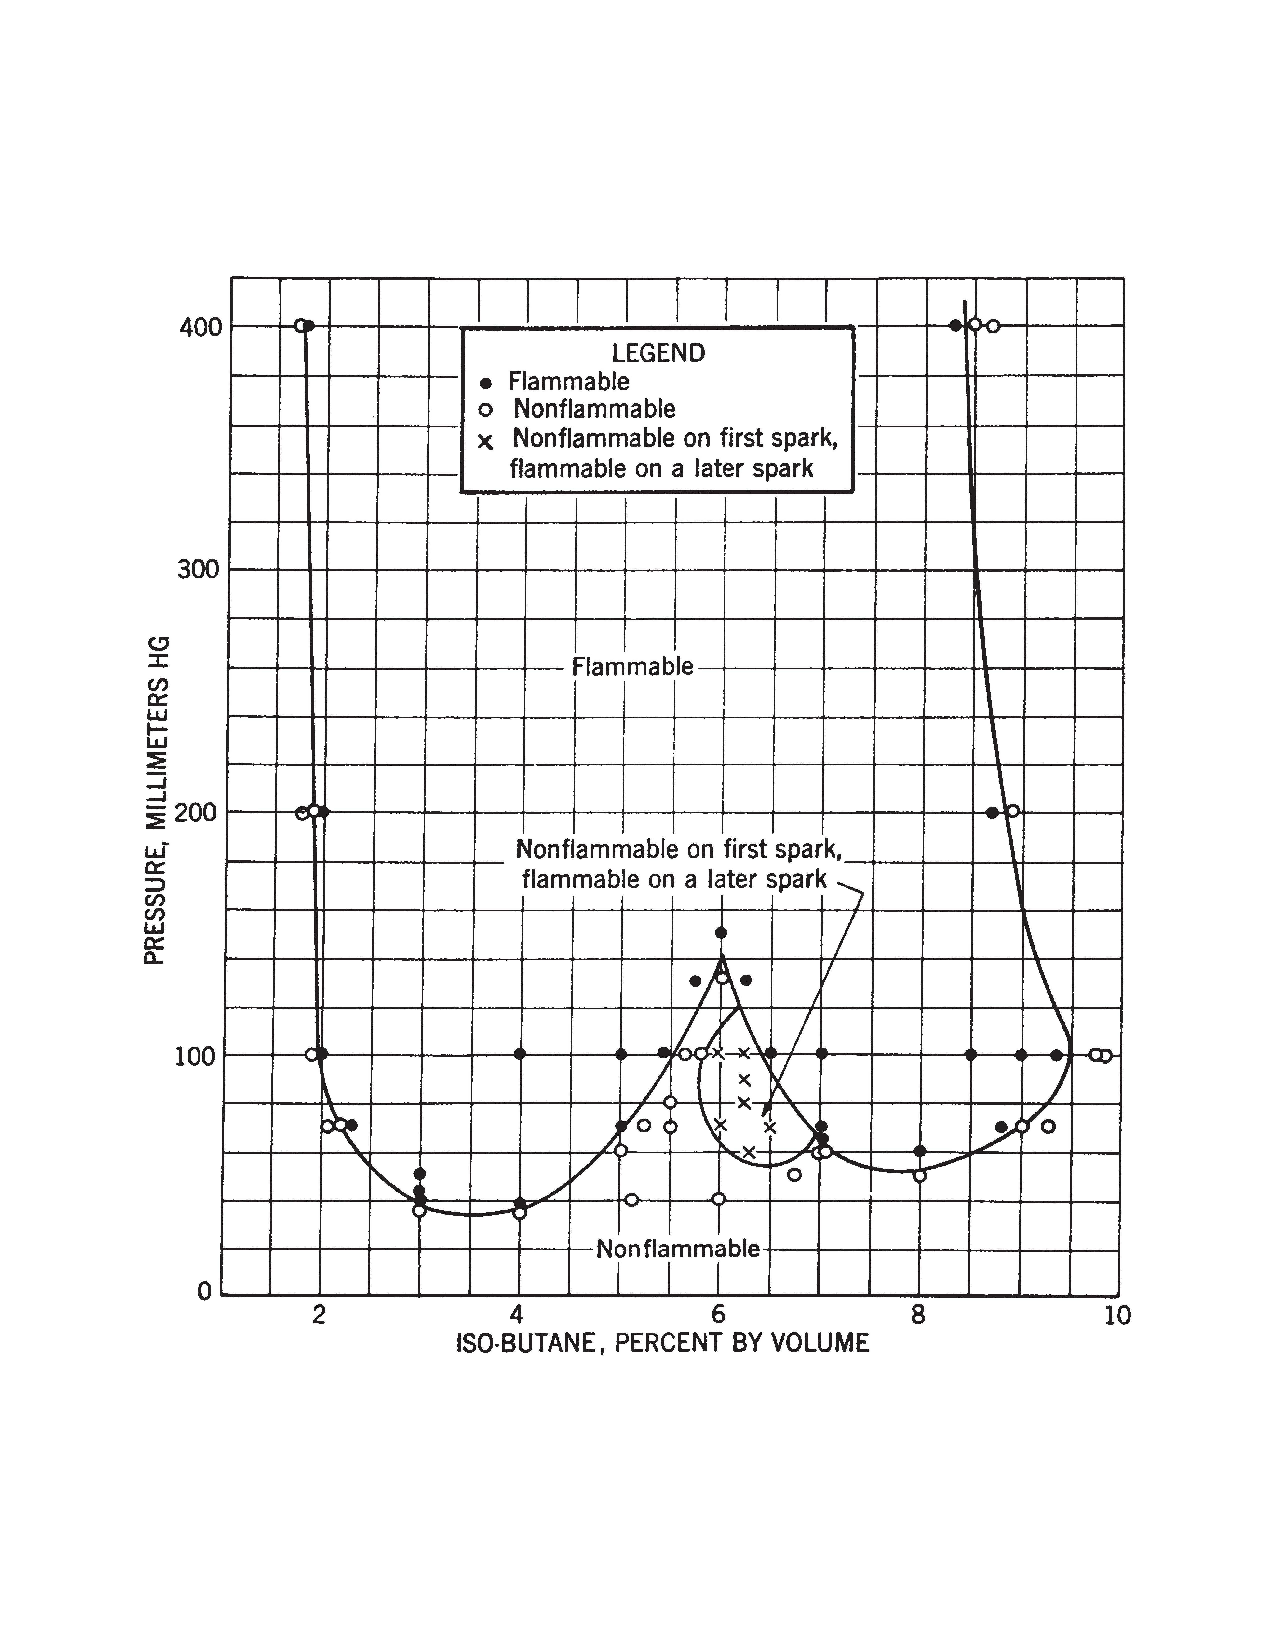
\includegraphics[width=\textwidth,height=0.5\textheight,keepaspectratio]{Scott_1952-fig7c}%
\caption{Flammability of isobutane at subatmospheric pressure.
%(Left) Figure from Ref.~\cite[Fig.~1]{Jones_1947}. (Right) %Flammability at subatmosphereic pressure.
Below 140\,Torr, the flammability limit becomes double-valued.  Below 40\,Torr, no concentration of isobutane is flammable.  Figure taken from Ref.~\cite[Fig.~7]{Scott_1952}}%
\label{lowpres}%
\end{figure}

\subsubsection{Pressure Change}
\paragraph{Isobutane} The possible increase in pressure due to combustion is the main hazard arising from the use of isobutane.  The rate of pressure increase and magnitude of the peak-to-initial pressure ratio is a minimum at the flammability limits and at a maximum near the stoichiometric ratio \cite{Zabetakis_1965}.
At standard temperature and pressure, the maximum flame propagation speed during the combustion of isobutane is about 36.7\,cm/s \cite{Davis_1998}.  This flame speed is well below the speed of sound (34,029\,cm/s), making the explosion a deflagration, as opposed to a detonation.  The peak flame speed occurs at an equivalence ratio of $\phi=1.1$.

A typical value of the peak-to-initial pressure ratio for the confined deflagration of a hydrocarbon is 8:1 \cite{Zabetakis_1965}.  This value can be calculated using the ideal gas law by taking the ratio of the adiabatic flame temperature of the combustion to the initial ambient temperature.  A number of studies have also determined this value empirically.
A somewhat dubious report published in Ref.~\cite{Zgliczynski_1994} claims a maximum peak-to-initial pressure ratio of 7.75 occurring at isobutane concentration of 3.5\%.  This concentration corresponds to an equivalence ratio of $\phi=1.12$ and a fuel-to-air ratio of 1:27.6.

\paragraph{$n$-butane} Ref.~\cite{Razus_2007} presents an extensive measurements of the pressure evolution of $n$-butane and air mixtures over a range of initial pressures and concentrations using different test chambers.  The maximum peak-to-initial pressure ratio and the maximum rate of pressure increase occur at a volume concentrations of 3.63\%.  This corresponds to an equivalence ratio of $\phi=$1.16, slightly above the stoichiometric ratio, and a fuel-to-air ratio of 1:26.5.  The maximum explosive pressure ratio measured was 9.34:1 for a spherical chamber and 9.01 for a cylindrical chamber.

Note that data for $n$-butane may be substituted  for isobutane in some cases.  For example, isobutane and $n$-butane, being chemical isomers, have the same molecular weight, specific gravity, and stoichiometric concentrations.
The flammability limits of the alkane hydrocarbons vary as a function of their molecular weight \cite{Zabetakis_1965}.  Consequently, studies of the flammability limits of $n$-butane are applicable to isobutane.  Additionally, Ref.~\cite{Davis_1998} shows that $n$-butane and isobutane have maximum flame speed at the same equivalence ratio.  The flame speed of $n$-butane reported in Ref.~\cite{Davis_1998} is about 40.8\,cm/s, or 111\% of the flame speed of isobutane.  Given that flame speed and explosion pressure are intimately related, the peak-to-initial pressure ratio of isobutane should be approximately 89.0\% of that reported for $n$-butane.  This assumption corresponds to an explosive pressure ratio for isobutane of %8.1--
8.4:1.

\paragraph{Shape dependence} As mentioned, the pressure evolution during an explosion depends on the shape of the chamber.  The time to peak pressure is proportional to the cube-root of the volume of the chamber \cite{Zabetakis_1965}. Based on the 12.6\,L volume of the PGAC box, the peak pressure should take approximately 57.3\,ms to develop.  However, this approximation assumes either spherical or cylindrical symmetry.  The parallelpiped configuration of the PGAC box may inhibit the production of pressure waves and reduce the maximum explosive pressure.


\subsection{Leak Scenarios}
%Potential sources of a leak are as follows.
\subsubsection{Worst-case scenario}
The worst-case would be the ignition of a near-stoichiometric mixture ($\phi=1.16$) of air and isobutane at atmospheric pressure  inside the confined volume  of the PGAC box. %, with the diagnostic box at atmospheric pressure.
This scenario requires a leak into the chamber to introduce air in a ratio of 26.5:1 to isobutane, resulting in a 3.63\% volume concentration of isobutane.  This concentration would produce a maximum explosive pressure of 6,380\,Torr (8.4\,atm) %8.51\,bar
inside the volume of the PGAC box.
%(30\,mbar iBu + 983\,mbar air),(1.5\,L)

If this scenario did occur, the resulting pressure increase would cause %at least one of the two 
the Mylar window to burst 
%at 24\,Torr differential pressure 
and vent the gasses into the 50\,L volume of the $0^{\circ}$ scattering chamber. The initial pressure in the scattering chamber would necessarily have been 760\,Torr %1.01\,bar
since the PGAC window can only support 57\,Torr of %limited
 differential pressure. The resulting maximum pressure in the combined volume would be
 1,890\,Torr (2.49\,atm or 1.49\,atm gauge pressure).
 %2.52\,bar (1.51\,bar gauge pressure).
 It should be noted that the Mylar window would break before the peak explosive pressure in the PGAC box could be reached.  The resulting dilution of the gas mixture would rapidly bring the concentration of isobutane below the flammability limit and quench flame propagation.

In reality, this scenario would be extremely difficult to achieve. The PID controller turns off the isobutane supply at pressures greater than its setpoint, which has a maximum value of of 10\,Torr.  Additional interlocks shut off the isobutane flow and the HV power if the diagnostic box pressure exceeds $\textrm{P}_\textrm{max}=7\times10^{-5}$\,Torr.  The required simultaneous, rapid influx of air filling the independent volumes of the PGAC box and the scattering chamber would almost certainly rupture the PGAC window and trip pressure interlocks that turn off the HV.  Even if HV interlocks failed and the bias was left constant, the increasing gas pressure would rapidly raise the breakdown voltage above the bias voltage, removing the source of ignition. %\cite{Heylen_1956}

\subsubsection{Low-pressure scenarios}
\label{low_pres}
\paragraph{UFL} A less contrived version of the worst-case scenario, i.e., one that does not require the simultaneous failure of multiple interlocks, would be an % massive
air leak into the volume of the PGAC box which is initially filled with 6\,Torr of isobutane.  With such a leak, %an air leak into isobutane, 
a flammable mixture would first form at the UFL when the concentration of isobutane is reduced to 8.43\%.  The fuel-to-air ratio of this mixture is 1:10.9.  The flow rate of isobutane into the detector is typically set at 60\,cc/min.
%0.10 Standard Liters per Minute (SLPM). 
 Assuming an air leak is already present when the detector gas flow was set, this would require a minimum air leak of 651\,cc/min
% 1.09\,SLPM
to form a combustible mixture.  

At the UFL, the total initial pressure in the PGAC box would be 71.2\,Torr. %142
  It is plausible %, however unlikely,
that the Mylar window could tolerate a pressure differential this high long enough to produce a flammable mixture.  If the flammable mixture was ignited, the resulting explosion would burst the Mylar window.  Since the explosion would be occurring at the limit of flammability, the peak-to-initial explosion pressure would be less than the maximum of 8.4:1.  Extrapolating from measurements with butane \cite{Razus_2007} and comparing to data for hydrogen \cite{Dahoe_2005}, at an equivalence ratio of $\phi=2.7$ the peak-to-initial explosion pressure ratio would be about 6.4:1.  Such an explosion would produce a maximum pressure in the combined  volume of the PGAC box and the scattering chamber of 91.7\,Torr. %183
% If the scattering chamber was also at an initial pressure of 71.2\,Torr, the final pressure of the system would be 149\,Torr.

\paragraph{Stoichiometric mix} An air leak leading to a stoichiometric gas mixture would have a higher explosion pressure.  However, in order to reach the stoichiometric fuel-to-air ratio of 1:31.0, a sustained air leak of 
1,860\,cc/min
%3.10\,SLPM
 would be required.  At the stoichiometric ratio, the pressure in the PGAC box would be 
 192\,Torr. %384
   This pressure is %near the upper limited of the estimated 
 so far above the
 burst pressure of the Mylar window that %, therefore
 it is unlikely that this gas mixture could be contained in the volume of the PGAC box.  Once dispersed into the 50\,L volume of the $0^\circ$ scattering chamber, the pressure of the gas mixture would be reduced to 38.7\,Torr %77\,Torr.  The resulting explosion would raise the pressure in the combined volume of the PGAC box and the scattering chamber to 495\,Torr.
 and ignition would be impossible.
 %Similarly, if the PGAC was operated at pressures above 6\,Torr, flammable gas mixtures could only be formed after the Mylar window has burst.

\paragraph {LFL}A scenario in which the PGAC box is accidentally vented would produce an even higher flow rate of air into the chamber.  However, such a leak  could only produce a gas mixture at or near the stoichiometric ratio for the reasons just discussed.  Namely, the Mylar window would break before a fuel-lean air mixture could be achieved.  Starting with an initial pressure of 6\,Torr of isobutane, % in the PGAC chamber, 
the LFL would be reached when the pressure in the PGAC box reached 328\,Torr. %656
 If this mixture were ignited, the resulting pressure in the combined volume of the PGAC box and the scattering chamber would be 422\,Torr. %845
   The analogous scenario resulting from the accidental venting of the scattering chamber could not produce a flammable mixture.  The pressure in the 50\,L scattering chamber required to burst the Mylar window would produce a gas mixture far below the LFL.

\subsubsection{Bellows damage }
A rupture in the beam line or the pumping system could cause an air leak into the chamber.  The most delicate component of these systems is the upstream bellows.  However, damage to the bellows is highly unlikely because the stable support of the chamber prevents any
mechanical stresses being applied to the bellows.

\subsubsection{Valve failure }
The only valves that ultimately open to air are in the roughing line and the venting line.  This would
require the simultaneous failure of 2--3 valves as show in Eq.~\ref{valve_fail}.  It should be noted that all of these combinations include at least one automatic valve which closes in the event of a power failure. % An air leak would require failure of the fail-safe.
In addition, if the pump valve was part of the failure, the roughing pump itself would also have to fail.  The coincidental failures required for a leak in the roughing line or the venting line is unlikely.

\begin{equation}
[\texttt{HEBTBV19} \lor (\texttt{HEBTRV19} \land \texttt{HEBTVV19A})] \land  (\texttt{HEBTTPV19} \lor \texttt{HEBTRV19})
\label{valve_fail}
\end{equation}

\subsubsection{Gas line damage (low pressure)}
If a leak develops the sub-atmospheric portion of the plumbing, the gas handling system will automatically decrease the detector gas flow rate to maintain the pressure. In this case, a far smaller leak would be needed to create a flammable mixture compared to a leak in the chamber.  With a total gas flow rate of 60\,cc/min,
%0.10\,SLPM,
an air leak of a 55\,cc/min
% 0.09\,SLPM
would be needed to create a combustible ratio mixture.  This is still a larger leak than one would expect from the Swagelok gas fittings used on the outside
of the chamber. Additionally, the flow rate of isobutane would visibly drop by 92\% from %0.10\,SLPM to 0.01\,SLPM,
60\,cc/min to 5.0\,cc/min,
which would trigger interlocks as detailed in \S~\ref{interlocks}.  It should be noted that at an operating pressure of 6\,Torr, this mixture would still not be flammable.

All sections of gas tubing which might be at sub-atmospheric pressure will be robust against
breakage. In particular, the tubing between \texttt{FC1} and the PGAC box; between the PGAC box, the scattering chamber, and valve
\texttt{VB4}; and between the gas supply panel and \texttt{VA1} should all be copper or stainless steel piping.
When possible, the roughing lines and will be located underneath the support structure which will act to protect them from external influences. %Similarly, the window bypass lines will be routed underneath the chamber.
Hence, damage to the low-pressure gas lines is unlikely.

\subsubsection{Gas line damage (high pressure)}
Leaks of isobutane from the above-atmospheric pressure portion of the plumbing into the surrounding air are not considered a significant hazard.  The stainless steel and copper plumbing lines used for the gas supply and exhaust are leaked-checked.  In the event of a complete line rupture, the maximum possible isobutane flow rate into the hall is only 250\,cc/min.

The air in the ISAC-II hall is replaced with fresh air every 11\,minutes (up to 110 minutes, depending on the recycled air ratio).
Tests under similar conditions have shown that a continuous 400\,cc/min isobutane leak would result in a flammable volume of less than 2\,L extending less than 30\,cm from the source of the leak   \cite{Openshaw_2006}. Additionally, a flammable gas sensor will be installed near the experimental area to detected any gas
leaks out into the ISAC-II hall.  An air leak into a sub-atmospheric volume containing isobutane and an ignition source would present a more significant hazard.

\subsubsection{Power failure} In the event of a power failure, all valves close and HV power supplies in the chamber latch off. The
scroll pump on the gas line is equipped with a valve that will default to closed so the chamber will
not vent to air. Thus, loss of power is not considered a potential hazard.

\section{Safety Measures}
A number of safety measures are proposed in order to minimize the risks and effects of the hazards
described above.  The EMMA PGAC GHS is very similar to the gas handling systems used in the IRIS ionization chamber, the MAYA PPAC, and the York PGAC.
\subsection{Hardware}
\begin{enumerate}
\setlength{\itemsep}{0pt}
\setlength{\parskip}{0pt}
\setlength{\parsep}{0pt}

\item The maximum flow of isobutane from the ISAC gas shack is limited to 250\,cc/min by a low-pressure regulator feeding gas through a pre-set needle valve.
\item A flammable gas sensor wired to an alarm in the main control room will be installed near the experimental area to detected any gas
leaks.
\item To prevent air-isobutane mixtures, isobutane is provided and pumped-out using the gas system plumbing only, whereas air is provided and pumped-out using the vacuum system plumbing only. To the extent possible, this is determined by the gas system design and enforced by interlocks.
\item The procedures specified in \S\,\ref{procedures} require all gas-containing volumes to be purged of air or pumped to vacuum, and leak tested before introducing isobutane flow to the PGAC box.
%\item  Two valves---one \marnote{missing $\rightarrow$} manual and one EPICS remote---will be installed in series on all gas lines entering the chamber to safeguard against failure leading to air ingress.
%\item Flammable materials near the chamber must be limited to essential materials only.
%\item To avoid a possible source of ignition, a cold cathode vacuum gauge is used to measure the scattering chamber pressure.
\item A dedicated gas system proportional-integral-differential (PID) controller will control the isobutane flow into the PGAC box to maintain the set pressure. 
\item The HV power supplies will be operated in trip-hold mode, ensuring that, at most, only one spark can occur.
\item All valves are normally closed (N/C) types. They will close on loss of electrical power. Air-actuated valves will also close on loss of air pressure.

\end{enumerate}
\subsection{Interlocks}
\label{interlocks}
The pressure within the volume of the PGAC box will be monitored throughout the experiment. If
the volumetric flow rate changes due to the development of a leak or a burst window, interlocks will be
triggered to make the chamber safe. The specific interlocks are as follows:
\begin{enumerate}
\item \texttt{VA1} can be open if and only if \texttt{HEBT:IG19} $<$ $\textrm{P}_\textrm{max}$.

This interlock shuts off the isobutane supply if the pressure in the scattering chamber exceeds $\textrm{P}_\textrm{max}$, typically set to $7\times10^{-5}$\,Torr.  This could occur in the event of isobutane entering the  scattering chamber via a broken window or if  bypass valve\texttt{VB4}   is opened with isobutane in PGAC box, etc.
\item The HV supply can be on if and only if 
(\texttt{VA1\_open}$) \land ($\texttt{FC1} $<\textrm{Q}_\textrm{max}) \land ($\texttt{FC1} $> \textrm{Q}_\textrm{min})$

The \texttt{VA1\_open} condition ensures the potential for gas flow and ensures that the  HV supply is off when \texttt{VA1} is tripped closed. % by window breakage or \texttt{VB4} being opened.
 It also
ensures that HV is off during pumping and venting operations.

The $\textrm{Q}_\textrm{min} < $ \texttt{FC1} $ < \textrm{Q}_\textrm{max}$ condition protects against air leaking into the the PGAC box after gas flow has
been established.
If air leaks into the PGAC box, the PID will reduce \texttt{FC1} flow to keep \texttt{PA1} pressure
constant.
As long as $\textrm{Q}_\textrm{max}/\textrm{Q}_\textrm{min} \lesssim 5$ , the volumetric flow rate will fall below Q$_\textrm{min}$ and trip off the HV before a
flammable mix of air and isobutane can be formed.  For example, the leak scenario detailed in \S\ref{low_pres} requires a ratio of $\textrm{Q}_\textrm{max}/\textrm{Q}_\textrm{min} =10.9$.  Typical values are Q$_\textrm{max}=100$\,cc/min, and  Q$_\textrm{min}=20$\,cc/min.
\end{enumerate}

\noindent Additionally, the solenoid valve on the pump \texttt{PU1} automatically shuts when the pump is turned off.
\subsection{Commissioning}
Prior to the experiment, a commissioning phase will be undertaken to investigate the various
features of the system. During this period the interlocks will be tested by initiating pressure rises
using an inert gas, e.g., nitrogen. %This will enable us to set high/low pressure interlocks to within a tight margin of nominal operational pressure.
Throughout these tests, the accelerator will
be protected by a gate valve.
\subsection{Procedures}
\label{procedures}
To prevent a flammable gas mixture forming within the chamber during venting and filling,
the following procedures will be followed.
\subsubsection{Fill procedure}
The following initial conditions are assumed.  Valve \texttt{VA1} is closed by interlock and pump \texttt{PU1} has been turned off, closing the automatic valve.  With these two valves closed, the chamber volumes are isolated from the gas lines.  The gas supply lines from the gas shack have been purged with isobutane and both chamber volumes are filled with air.  Valve  \texttt{HEBT:BV19} is closed and the turbo pump is off. 
\begin{itemize}
\setlength{\itemsep}{0pt}
\setlength{\parskip}{0pt}
\setlength{\parsep}{0pt}
%\item Close \texttt{VB3} \marnote{missing $\rightarrow$} to seal the gas exhaust line, not used for air (this valve is not on the diagram)
\item Open bypass valve \texttt{VB4} between the PGAC box and the scattering chamber.
\item Open bypass valve \texttt{VB2} on the exhaust line to bypass exhaust needle valve \texttt{VN1}.
\item Close manual regulating valve \texttt{HEBT:MRV19} on the roughing line.   Ensure that roughing valve \texttt{HEBT:RV19} on the roughing line and ball valve \texttt{HEBT:BV19} on the turbo backing line are also closed.
\item Open pumping valve \texttt{HEBT:PV19} and roughing valve \texttt{HEBT:RV19} on the roughing line.
\item Adjust manual regulating valve \texttt{HEBT:MRV19}  while monitoring differential pressure on \texttt{PD1}.  The differential pressure should not exceed $\pm$4\,Torr.
\item Once the chambers are pumped out, close bypass valve \texttt{VB4} and close roughing valve \texttt{HEVT:RV19} to isolate the chambers.
\item Leak check both volumes by monitoring the independent pressure in each volume.  The pressures should be stable.
\item Open valve \texttt{HEBT:BV19}, start the turbo pump \texttt{HEBT:TP19}, and turn on ionization gauge \texttt{IG19}.
\item Set desired pressure on PID
\item Close bypass valve \texttt{VB2} on the gas exhaust line. %to bypass the gas flow rate valve \texttt{VN1}
\item Verify exhaust valve  \texttt{VB6} is open on the gas supply panel.
\item Turn on pump \texttt{PU1} to vent the exhaust.
\item Turn on flow control \texttt{FC1} and open vale \texttt{VA1} on the supply line to begin the gas flow.
\item Adjust needle valve \texttt{VN1} to obtain the desired flow-rate in \texttt{FC1} (nominally 60\,cc/min).  As the pressure \texttt{PA1} increases, open \texttt{VN1}. Wait until \texttt{PA1} and \texttt{FC1} are stable at their desired values.
\item Turn on HV power supplies, ramp the voltage to the desired value, and enabled current trip hold.
\item Open gate valve \texttt{HEBT:IV18} to the beam line
\end{itemize}
\subsubsection{Vent Procedure}
\begin{itemize}
\setlength{\itemsep}{0pt}
\setlength{\parskip}{0pt}
\setlength{\parsep}{0pt}
\item Close beam gate valve \texttt{HEBT:IV18} on the beam line.
\item Turn off turbo pump \texttt{HEBT:TP19}  and turn off ionization gauge \texttt{IG19}.
\item Turn off the HV power supplies and close valve \texttt{VA1} on the supply line.
\item Open flow rate bypass valve \texttt{VB2} to fully evacuate gas from the PGAC box.
\item Once \texttt{PA1} $\lesssim 1$\,Torr, turn off pump \texttt{PU1}, closing the automatic valve on the gas exhaust line, and open bypass valve \texttt{VB4}.
\item Close manual regulating valve \texttt{HEBT:MRV19} on the roughing line.   Ensure that the following valves are also closed: roughing valve \texttt{HEBT:RV19} on the roughing line, ball valve \texttt{HEBT:BV19} on the turbo backing line, and manual vent valve \texttt{HEBT:MVV19} on the venting line.
\item Open valve \texttt{HEBT:VV19} on the venting line.
\item Adjust the regulating vent valve \texttt{MVV19} on the venting line while monitoring \texttt{PD1}.  The differential pressure should not exceed $\pm$4\,Torr.
\end{itemize}
\subsubsection{Pressure Change Procedure}
\begin{itemize}
\setlength{\itemsep}{0pt}
\setlength{\parskip}{0pt}
\setlength{\parsep}{0pt}
\item Close gate valve \texttt{HEBT:IV18} on the beam line.
\item Turn off the HV power supplies.
\item Adjust the pressure on the PID controller.
\item Adjust needle valve \texttt{VN1} to desired flow-rate.  Wait until \texttt{PA1} and \texttt{FC1} are stable at their desired values.
\item Turn on HV power supplies, ramp the voltage to the desired value, and enabled current trip hold.
\item Open gate valve \texttt{HEBT:IV18} on the beam line
\end{itemize}
\subsubsection{Gas Alarm Procedure}
\begin{itemize}
\setlength{\itemsep}{0pt}
\setlength{\parskip}{0pt}
\setlength{\parsep}{0pt}

\item Close gate valve \texttt{HEBT:IV18} on the beam line.
\item Turn off the HV power supplies.
\item Close valve \texttt{VA1} on the gas supply line.
\item Turn off pump \texttt{PU1}, closing the automatic valve on the gas exhaust line.
\item Close valves \texttt{VB1} and \texttt{VB6} on the gas supply panel.
\item Contact Robert Openshaw or Philip Lu.
\end{itemize}
\subsubsection{Fire Alarm}
Follow the normal evacuation procedure and leave the area at once.
\section{Definition of Responsibilities}
The Experiment Leader is responsible for ensuring that during the experiment:
\begin{enumerate}
\setlength{\itemsep}{0pt}
\setlength{\parskip}{0pt}
\setlength{\parsep}{0pt}

\item  There is no unattended operation when detector is in use with gas.
\item  Everyone on shift has read and understood this report.
\item  Everyone on shift has demonstrated the procedures described in \S~\ref{procedures}.
\end{enumerate}
\section{Decommissioning or Disposal}
No non-standard decommissioning or disposal procedures are required following this experiment.

%\nocite{*}
\bibliographystyle{elsarticle-aps6} 
\bibliography{isobutane}
